\usepackage[utf8]{inputenc}
\usepackage{graphicx}
\usepackage{float}
\graphicspath{{graficos/}}
\usepackage{tikz}
\usetikzlibrary{calc}
\pgfdeclarelayer{background}
\pgfdeclarelayer{foreground}
\pgfsetlayers{background,main,foreground}
\usepackage{fontspec}
\setmainfont{Times New Roman} 
\usepackage{helvet}
\newfontfamily\arialbold{Arial Bold}
\usepackage{amsmath}
\usepackage{amsfonts}
\usepackage{ifthen}
\usepackage{tabularx}
%%%%%%%%%%%%%%%%%%%%%%%%%%%%%%%%%%%%%%%%%%%%%%%%%%%%%%%%%%
\usepackage[nonumberlist,automake]{glossaries}
% Generate the glossary 
\makeglossaries
%%%%%%%%%%%%%%%%%%%%%%%%%%%%%%%%%%%%%%%%%%%%%%%%%%%%%%%%%%
  \usepackage{colortbl}
  \definecolor{Lightgray}{RGB}{235,235,235}
%%%%%%%%%%%%%%%%%%%%%%%%%%%%%%%%%%%%%%%%%%%%%%%%%%%%%%%%%%
\setlength{\parskip}{6pt}
%%%%%%%%%%%%%%%%%%%%%%%%%%%%%%%%%%%%%%%%%%%%%%%%%%%%%%%%%%
\setcounter{tocdepth}{4}
\setcounter{secnumdepth}{4}
%%%%%%%%%%%%%%%%%%%%%%%%%%%%%%%%%%%%%%%%%%%%%%%%%%%%%%%%%%
\usepackage[
  inner	=	3.0cm, % Margen interior
  outer	=	3.0cm, % Margen exterior
  top	=	2.5cm, % Margen superior
  bottom=	2.5cm, % Margen inferior
  includeheadfoot, % Incluye cabecera y pie de página en los márgenes
]{geometry}
%\renewcommand{\baselinestretch}{1.0}
\usepackage{xcolor}
\usepackage{sectsty}
\chapterfont{\color{azul}}  % sets colour of chapters
\sectionfont{\color{azul}}  % sets colour of sections
\subsectionfont{\color{azul}}  % sets colour of sections
\subsubsectionfont{\color{azul}}  % sets colour of sections
%%%%%%%%%%%%%%%%%%%%%%%%%%%%%%%%%%%%%%%%%%%%%%%%%%%%%%%%
\usepackage[style=numeric,sorting=none]{biblatex}
\addbibresource{referencias.bib}
%%%%%%%%%%%%%%%%%%%%%%%%%%%%%%%%%%%%%%%%%%%%%%%%%%%%%%%%
\usepackage{booktabs}
\usepackage{threeparttable}
%%%%%%%%%%%%%%%%%%%%%%%%%%%%%%%%%%%%%%%%%%%%%%%%%%%%%%%%
\usepackage{tocloft}
\cftpagenumbersoff{part}
%%%%%%%%%%%%%%%%%%%%%%%%%%%%%%%%%%%%%%%%%%%%%%%%%%%%%%%%
\defbibheading{firstlevel}[]{%
    \chapter*{#1}
    \addcontentsline{toc}{chapter}{#1}}

%%%%%%%%%%%%%%%%%%%%%%%%%%%%%%%%%%%%%%%%%%%%%%%%%%%%%%%%
\usepackage[spanish]{babel}
%\usepackage[spanish]{polyglossia}
%\setdefaultlanguage{spanish}

% \addto\captionsspanish{%
% 	\renewcommand{\listtablename}{Índice de tablas} 
% 	\renewcommand{\tablename}{Tabla}
% 	\renewcommand{\lstlistingname}{Código}
% 	\renewcommand{\lstlistlistingname}{Índice de \lstlistingname s}
% 	\renewcommand{\glossaryname}{Glosario}
% 	\renewcommand{\acronymname}{Acrónimos}
% 	\renewcommand{\bibname}{Bibliografía}%
% }
%%%%%%%%%%%%%%%%%%%%%%%%%%%%%%%%%%%%%%%%%%%%%%%%%%%%%%%%
\usepackage{hyperref}
% Codigo QR del repositorio, en la introduccion. Se dibuja con TikZ, asi que no
% hace falta ninguna imagen externa ni herramienta fuera de LaTeX.
\usepackage{qrcode}
%%%%%%%%%%%%%%%%%%%%%%%%%%%%%%%%%%%%%%%%%%%%%%%%%%%%%%%%
\usepackage{fancyhdr}% http://ctan.org/pkg/fancyhdr
\pagestyle{fancy}% Change page style to fancy
\fancyhf{}% Clear header/footer
%\fancyhead[C]{Header}
\fancyhead[RO]{\footnotesize\color{azul}\rightmark}
\fancyhead[LE]{\footnotesize\color{azul}\leftmark}
\fancyfoot[C]{\footnotesize\color{azul} \thepage}% \fancyfoot[R]{\thepage}
\renewcommand{\headrulewidth}{0.4pt}% Default \headrulewidth is 0.4pt
\renewcommand{\footrulewidth}{0.4pt}% Default \footrulewidth is 0pt
\makeatletter
\renewcommand{\headrule}{\setlength\@tempdima{\headrulewidth}
\textcolor{azul}{\hrule\@height\@tempdima\@width\headwidth}
\vskip -2\@tempdima}
\makeatother
\renewcommand{\footrule}{\hbox to\headwidth{\color{azul}\leaders\hrule height \footrulewidth\hfill}}

% Redefine the plain page style
\fancypagestyle{plain}{%
  \fancyhf{}%
  \fancyfoot[C]{\footnotesize\color{azul} \thepage}%
  \renewcommand{\headrulewidth}{0pt}% Line at the header invisible
  \renewcommand{\footrulewidth}{0.4pt}% Line at the footer visible
}
%%%Acercar texto y línea en cabecera
\makeatletter
\def\headrule{{
  \if@fancyplain\let\headrulewidth\plainheadrulewidth\fi
  \vskip0pt% change here
  \color{azul}\hrule\@height\headrulewidth\@width\headwidth   
  \vskip-\headrulewidth%
}}
%%%%%%%%%%%%%%%%%%%%%%%%%%%%%%%%%%%%%%%%%%%%%%%%%%%%%%%%
%Part reinicia la numeración de capítulos
\makeatletter
\@addtoreset{chapter}{part}
\makeatother
%%%%%%%%%%%%%%%%%%%%%%%%%%%%%%%%%%%%%%%%%%%%%%%%%%%%%%%%
%Part sin numeración de página
\makeatletter
\renewcommand\part{%
  \if@openright
    \cleardoublepage
  \else
    \clearpage
  \fi
  \thispagestyle{empty}%   % Original »plain« replaced by »emptyx
  \if@twocolumn
    \onecolumn
    \@tempswatrue
  \else
    \@tempswafalse
  \fi
  \null\vfil
  \secdef\@part\@spart}
\makeatother
%%%%%%%%%%%%%%%%%%%%%%%%%%%%%%%%%%%%%%%%%%%%%%%%%%%%%%%%
%Pie de figura en negrita
\usepackage[font=footnotesize,labelfont=bf]{caption}
%%%%%%%%%%%%%%%%%%%%%%%%%%%%%%%%%%%%%%%%%%%%%%%%%%%%%%%%
%Colocacion de figuras: los valores por defecto de LaTeX son muy
%restrictivos y empujan las figuras a paginas posteriores
\renewcommand{\topfraction}{0.9}
\renewcommand{\bottomfraction}{0.7}
\renewcommand{\textfraction}{0.1}
\renewcommand{\floatpagefraction}{0.75}
\setcounter{topnumber}{3}
\setcounter{bottomnumber}{2}
\setcounter{totalnumber}{4}
\setlength{\intextsep}{12pt plus 4pt minus 4pt}
\setlength{\textfloatsep}{14pt plus 4pt minus 4pt}
%Impide que una figura se cuele en una seccion posterior a la que la cita
\usepackage[section]{placeins}
%%%%%%%%%%%%%%%%%%%%%%%%%%%%%%%%%%%%%%%%%%%%%%%%%%%%%%%%
%DESCOMENTAR para tener numeración de figuras y tablas 
%continua en todo el documento
%\renewcommand\thefigure{\arabic{figure}}
%\renewcommand\thetable{\arabic{table}}
%\renewcommand\theequation{\arabic{equation}}
%\setcounter{figure}{0}

%\usepackage{chngcntr}
%\counterwithout{figure}{chapter}
%\counterwithout{table}{chapter}
%counterwithout{equation}{chapter}

%%%%%%%%%%%%%%%%%%%%%%%%%%%%%%%%%%%%%%%%%%%%%%%%%%%%%%%%
%DESCOMENTAR PARA ELIMINAR EL INDENTADO INICIAL DE LOS PÁRRAFOS
\setlength{\parindent}{0pt}
%%%%%%%%%%%%%%%%%%%%%%%%%%%%%%%%%%%%%%%%%%%%%%%%%%%%%%%%


\raggedbottom

%-------------------------------------------------
%Creación de la tabla de RESUMEN EJECUTIVO

\newenvironment{tablaRE}{
\noindent\textbf{RESUMEN EJECUTIVO}
\comentarioRESUMEN
\noindent La memoria del \TFGTFM\ del \NOMBRETITULO\ debe desarrollar en el texto los siguientes conceptos, debidamente justificados y discutidos, centrados en el ámbito de la \NOMBREDISCIPLINA\ \\


\begin{tikzpicture}\node[coordinate] at (0,0) (origen){};}{
\end{tikzpicture}

\begin{tikzpicture}[overlay,remember picture]
\node[anchor=south west] at ($(current page.south west)+(16,1.5)$) {\parbox{10cm}{\footnotesize
Escuela Técnica Superior de Ingeniería de Telecomunicación\\
Universitat Politècnica de València\\
Edificio 4D. Camino de Vera, s/n, 46022 Valencia\\
Tel. +34 96 387 71 90, ext. 77190\\
\textbf{www.etsit.upv.es}
}};
\node[anchor=south] at ($(current page.south west)+(30,1.25)$) {
\includegraphics[width=8cm]{graficos/logos.png}};
\node[anchor=north west] at ($(current page.center)+(5,6)$) {
\includegraphics[scale=0.5]{graficos/marca_UPV_principal_negro.pdf}};
\node[anchor=north west] at ($(current page.center)+(15,6)$) {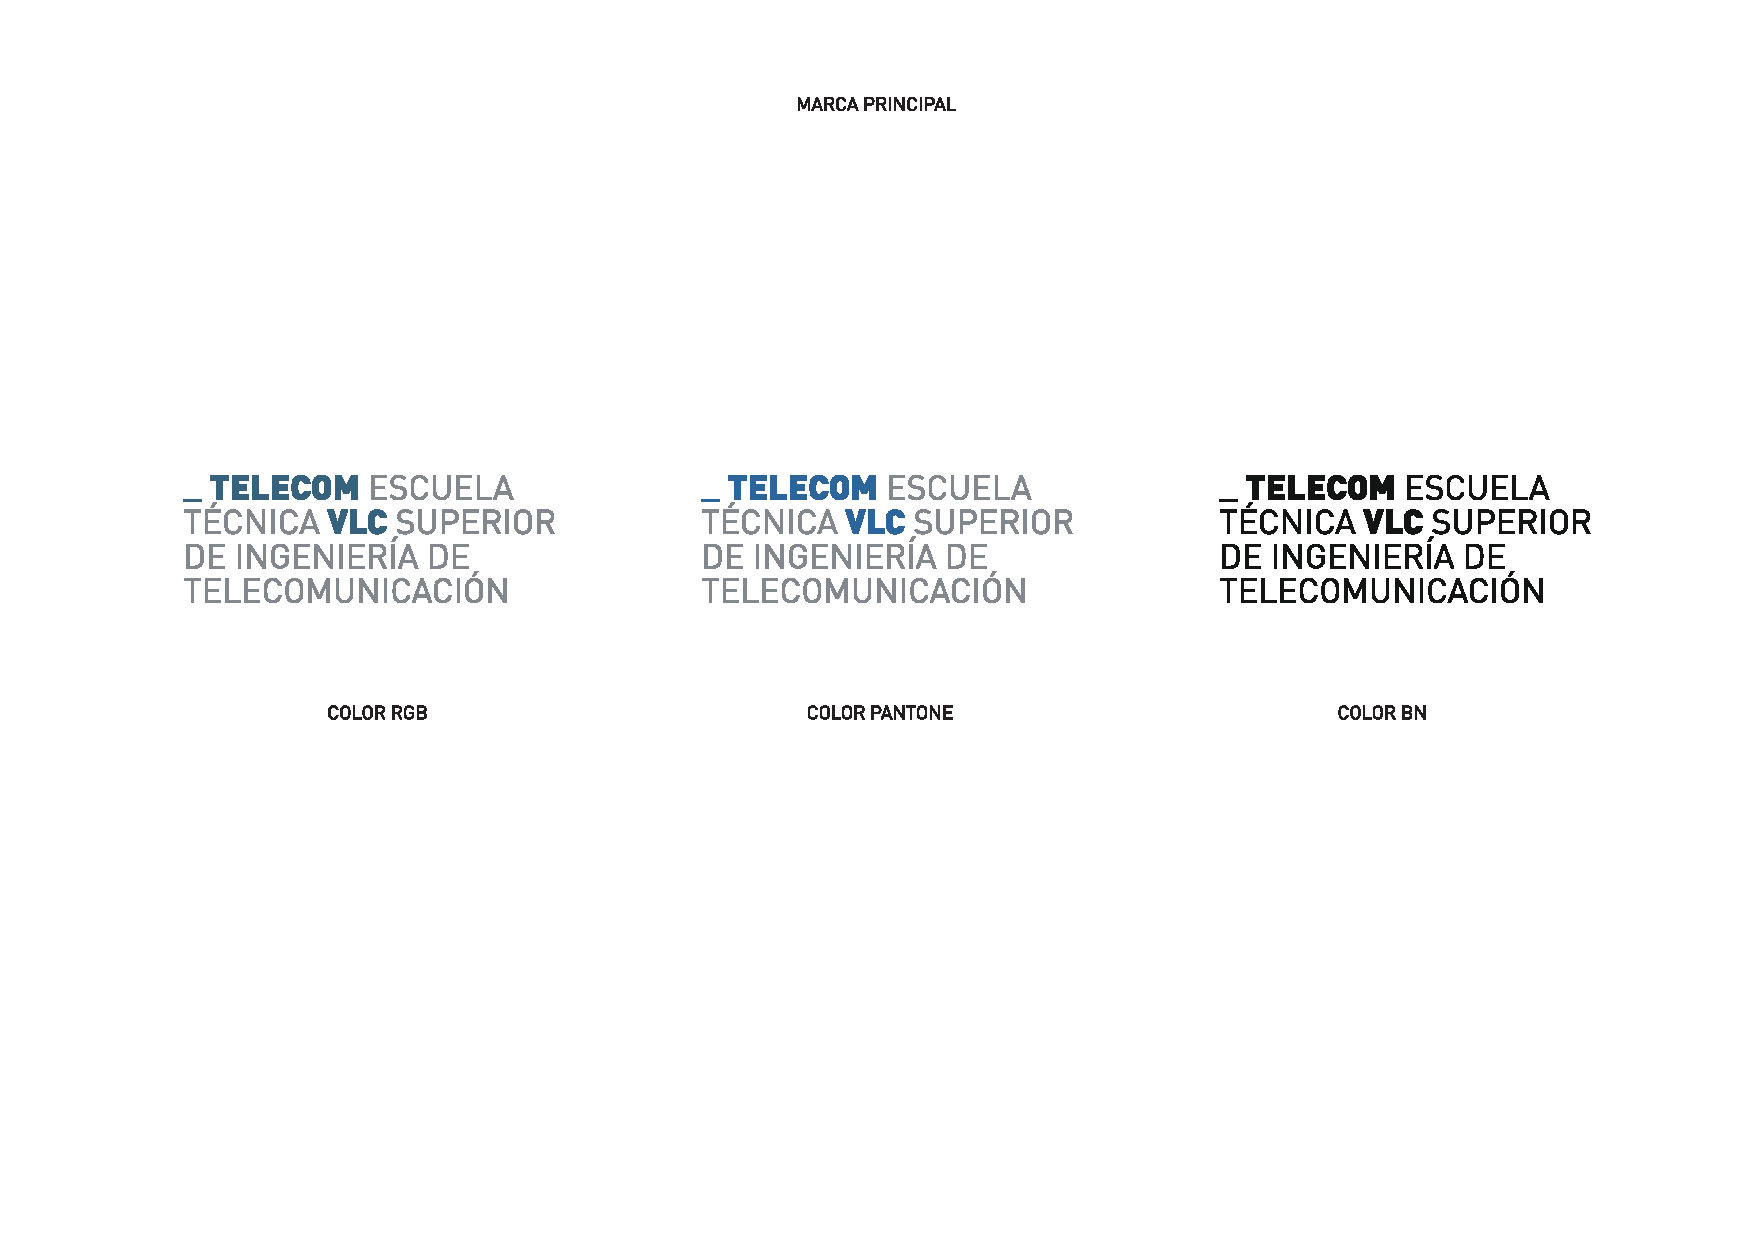
\includegraphics[scale=0.55,trim=10cm 10.7cm 10cm 8cm,clip]{graficos/2018_TELECOMVLC.pdf}};
\end{tikzpicture}
}


\usepackage{pdflscape}

\def\anchocolA{8cm}
\def\anchocolB{8cm}
\def\anchocolC{2cm}
\def\anchocolD{2cm}
\newcommand{\cabecera}[5]{%
  \newlength{\ajuste}
  \setlength{\ajuste}{3mm}
  \node[draw=lightgray,anchor=north west,minimum width=\anchocolA,,minimum height=#1] at (origen.south) (colA) {\parbox{\anchocolA}{\ifthenelse{\equal{\unexpanded{#2}}{}}{\ }{\raggedright \bf#2}}};
  \node[coordinate] (origen) at (colA.south west){};
  \node[draw=lightgray,anchor=north west,minimum width=\anchocolB,,minimum height=#1] at (colA.north east) (colB) {\parbox{\anchocolB}{\ifthenelse{\equal{\unexpanded{#3}}{}}{\ }{\raggedright \bf#3}}};
  \node[draw=lightgray,anchor=north west,minimum width=\anchocolC,,minimum height=#1] at (colB.north east) (colC) {\parbox{\anchocolC}{\ifthenelse{\equal{\unexpanded{#4}}{}}{\ }{\centering\bf#4}}};
  \node[draw=lightgray,anchor=north west,minimum width=\anchocolD,,minimum height=#1] at (colC.north east) (colD) {\parbox{\anchocolD}{\ifthenelse{\equal{\unexpanded{#5}}{}}{\ }{\centering \bf#5}}};
  
  \node[coordinate] at (colA.north west) (L1){};
  \node[coordinate] at (colA.south west) (L2){};
  \node[coordinate] at (colD.north east) (R1){};
  \node[coordinate] at (colD.south east) (R2){};
}%
\newcommand{\fila}[5]{%
  \node[draw=lightgray,anchor=north west,minimum width=\anchocolA,,minimum height=#1] at (origen.south) (colA) {\parbox{\anchocolA}{\ifthenelse{\equal{\unexpanded{#2}}{}}{\ }{\raggedright #2}}};
  \node[coordinate] (origen) at (colA.south west){};
  \node[draw=lightgray,anchor=north west,minimum width=\anchocolB,,minimum height=#1] at (colA.north east) (colB) {\parbox{\anchocolB}{\ifthenelse{\equal{\unexpanded{#3}}{}}{\ }{\raggedright #3}}};
  \node[draw=lightgray,anchor=north west,minimum width=\anchocolC,,minimum height=#1] at (colB.north east) (colC) {\parbox{\anchocolC}{\ifthenelse{\equal{\unexpanded{#4}}{}}{\ }{\centering #4}}};
  \node[draw=lightgray,anchor=north west,minimum width=\anchocolD,,minimum height=#1] at (colC.north east) (colD) {\parbox{\anchocolD}{\ifthenelse{\equal{\unexpanded{#5}}{}}{\ }{\centering #5}}};
}
\newcommand{\pie}[5]{%
  \node[draw=lightgray,anchor=north west,minimum width=\anchocolA,,minimum height=#1] at (origen.south) (colA) {\parbox{\anchocolA}{\ifthenelse{\equal{\unexpanded{#2}}{}}{\ }{\raggedright #2}}};
  \node[coordinate] (origen) at (colA.south west){};
  \node[draw=lightgray,anchor=north west,minimum width=\anchocolB,,minimum height=#1] at (colA.north east) (colB) {\parbox{\anchocolB}{\ifthenelse{\equal{\unexpanded{#3}}{}}{\ }{\raggedright #3}}};
  \node[draw=lightgray,anchor=north west,minimum width=\anchocolC,,minimum height=#1] at (colB.north east) (colC) {\parbox{\anchocolC}{\ifthenelse{\equal{\unexpanded{#4}}{}}{\ }{\centering #4}}};
  \node[draw=lightgray,anchor=north west,minimum width=\anchocolD,,minimum height=#1] at (colC.north east) (colD) {\parbox{\anchocolD}{\ifthenelse{\equal{\unexpanded{#5}}{}}{\ }{\centering #5}}};
  \node[coordinate] at (colA.south west) (L3){};
  \node[coordinate] at (colD.south east) (R3){};
  \draw[black,thick] (L1) rectangle (R2);
  \draw[black,thick] (L2)  rectangle (R3);
}


%%%%%%%%%%%%%%%%%%%%

